% TU Delft Beamer template
% Author: Maarten Abbink
% Delft University of Technology
% March 2014
% Version 2.0
% Based on original version 1.0 of Carl Schneider
\documentclass{beamer}
\usepackage[english]{babel}
\usepackage{calc}
\usepackage[absolute,overlay]{textpos}
\mode<presentation>{\usetheme{tud}}

\title[OBFN]{Master Thesis}
\subtitle {Tuning of the Optical Beamforming Networks}
\institute[TU Delft]{Delft University of Technology}
\author{Herminarto Nugroho}
\date{\today}

% Insert frame before each subsection (requires 2 latex runs)
%\AtBeginSubsection[] {
%	\begin{frame}<beamer>\frametitle{\titleSubsec}
%		\tableofcontents[currentsection,currentsubsection]  % Generation of the Table of Contents
%	\end{frame}
%}
% Define the title of each inserted pre-subsection frame
\newcommand*\titleSubsec{Next Subsection}
% Define the title of the "Table of Contents" frame
\newcommand*\titleTOC{Outline}

% define a symbol which can be removed if you don't need it
\newcommand{\field}[1]{\mathbb{#1}}
\newcommand{\Zset}{\field{Z}}

\begin{document}

{
% remove the next line if you don't want a background image
%\usebackgroundtemplate{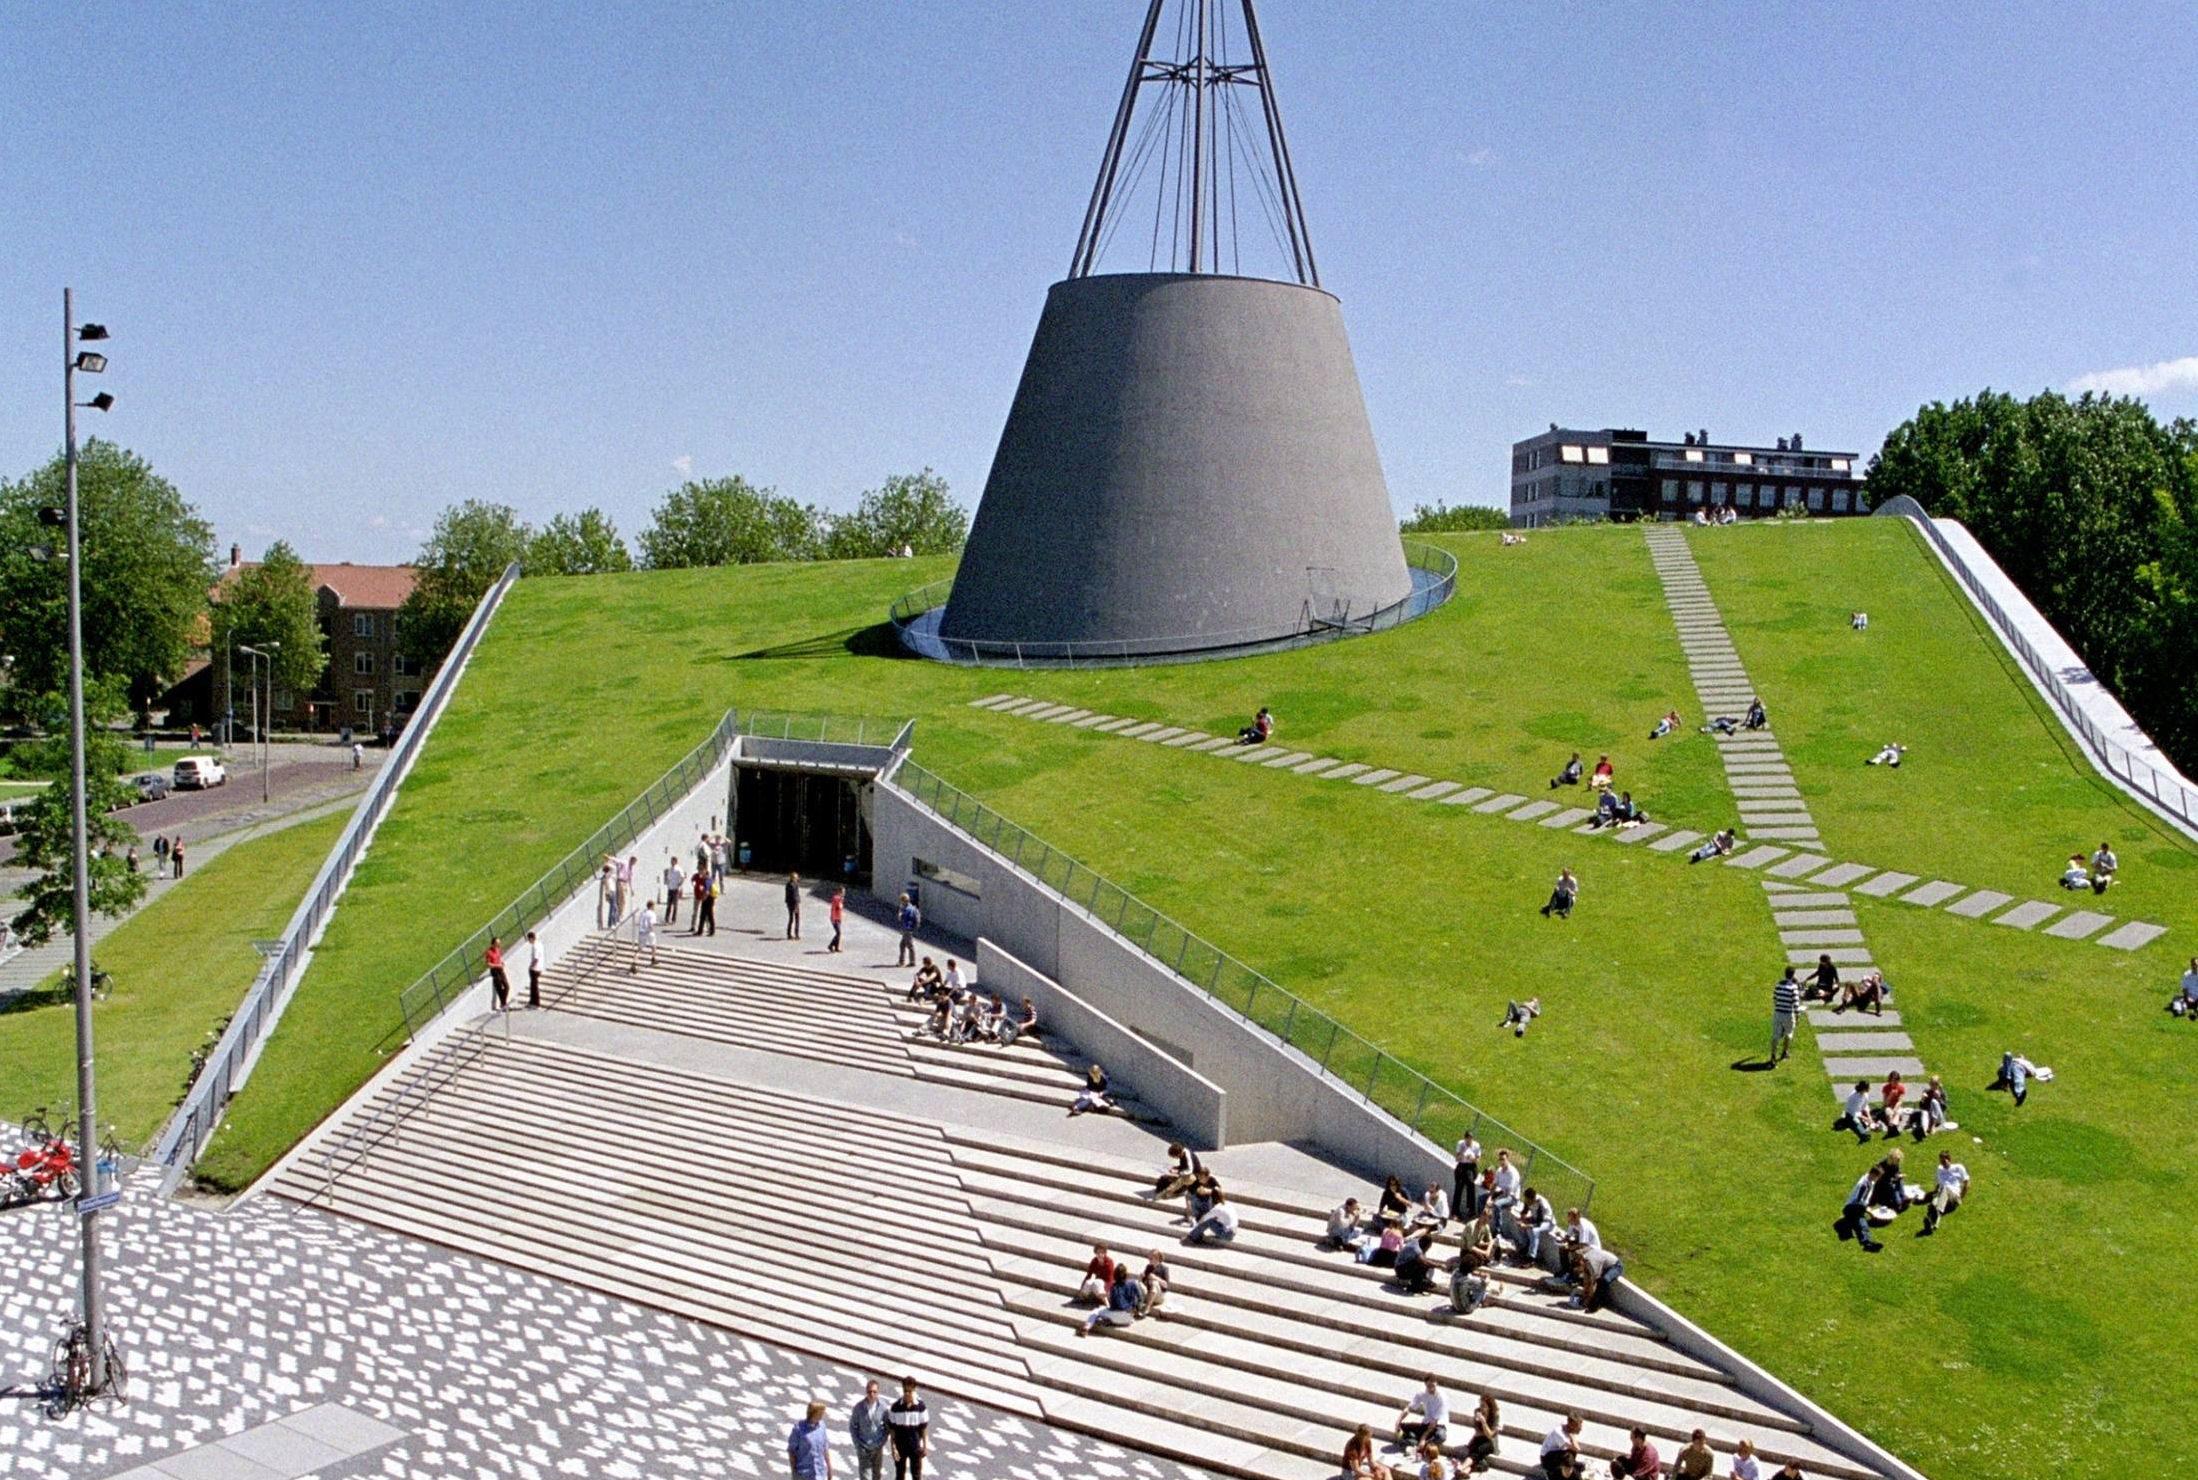
\includegraphics[width=\paperwidth,height=\paperheight]{images/background-titlepage.jpg}}%
\setbeamertemplate{footline}{\usebeamertemplate*{minimal footline}}
\frame{\titlepage}
}

{\setbeamertemplate{footline}{\usebeamertemplate*{minimal footline}}
\begin{frame}\frametitle{\titleTOC}
	\tableofcontents
\end{frame}
}

\section{Project Description}
\subsection{Project Overview}

\begin{frame}\frametitle{Project Overview}
	%\begin{example}
		%\begin{minipage}{0.6\textwidth}
			% insert picture (pdf file)
			%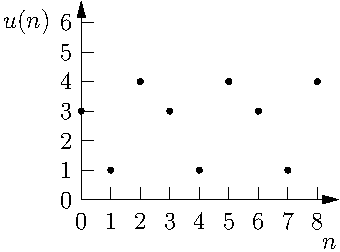
\includegraphics{images/ex1_periodic_number.pdf}
		%\end{minipage}
		%\centering{$u(n)=[3,1,4]_n$}
	%\end{example}
	
	\begin{figure}[H]
	\begin{minipage}[t]{0.45\textwidth}
	\centering
	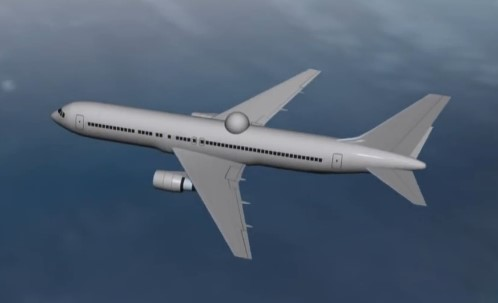
\includegraphics[width=\linewidth]{images/past_antenna}
	\caption{Step response of open loop}
	\label{fig:bandwidth1}
	\end{minipage}
	\hspace{\fill}
	\begin{minipage}[t]{0.45\textwidth}
	\centering
	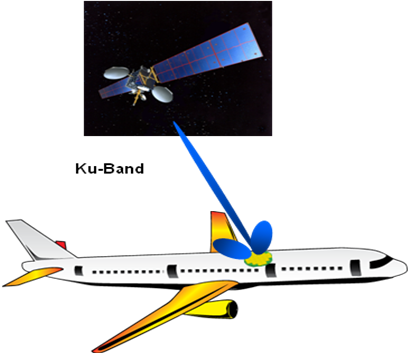
\includegraphics[width=\linewidth]{images/satrax_plane}
	\caption{Delay estimation}
	\label{fig:bandwidth2}
	
	\end{minipage}
	\end{figure}
	
\end{frame}

\begin{frame}\frametitle{Project Overview}
	\begin{figure}[H]
		\begin{minipage}[t]{0.45\textwidth}
			\centering
			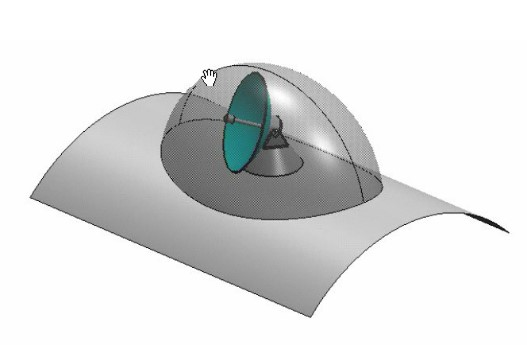
\includegraphics[width=\linewidth]{images/past_antenna1}
			\caption{Step response of open loop}
			\label{fig:bandwidth1}
		\end{minipage}
			\hspace{\fill}
		\begin{minipage}[t]{0.45\textwidth}
			\centering
			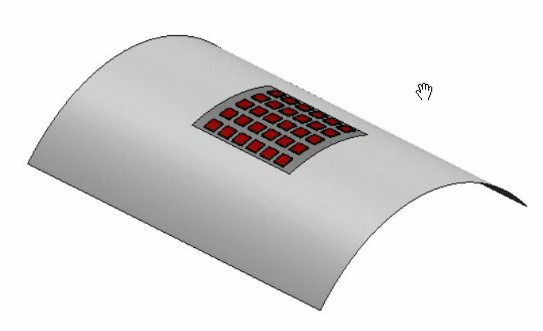
\includegraphics[width=\linewidth]{images/paa_1}
			\caption{Delay estimation}
			\label{fig:bandwidth2}
		\end{minipage}
	\end{figure}
\end{frame}

\subsection{Phased Array Antennas}

\begin{frame}\frametitle{Phased Array Antennas}
		\begin{figure}
			\centering
			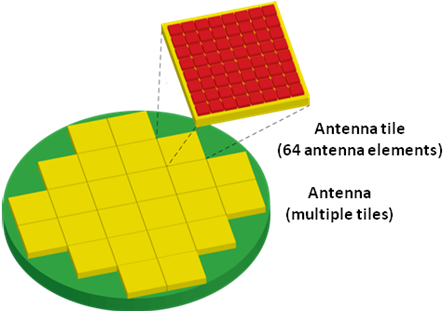
\includegraphics[width=0.3\linewidth]{images/satrax_antenna}
			\caption{Step response of open loop}
			\label{fig:bandwidth1}
		\end{figure}
		\begin{figure}[H]
			\begin{minipage}[t]{0.45\textwidth}
				\centering
				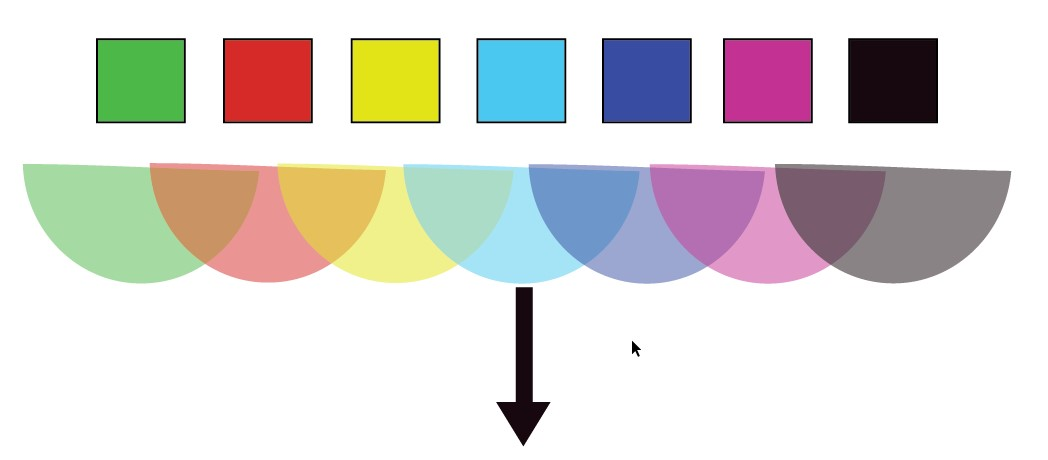
\includegraphics[width=\linewidth]{images/paa_straight}
				\caption{Step response of open loop}
				\label{fig:bandwidth1}
			\end{minipage}
				\hspace{\fill}
			\begin{minipage}[t]{0.45\textwidth}
				\centering
				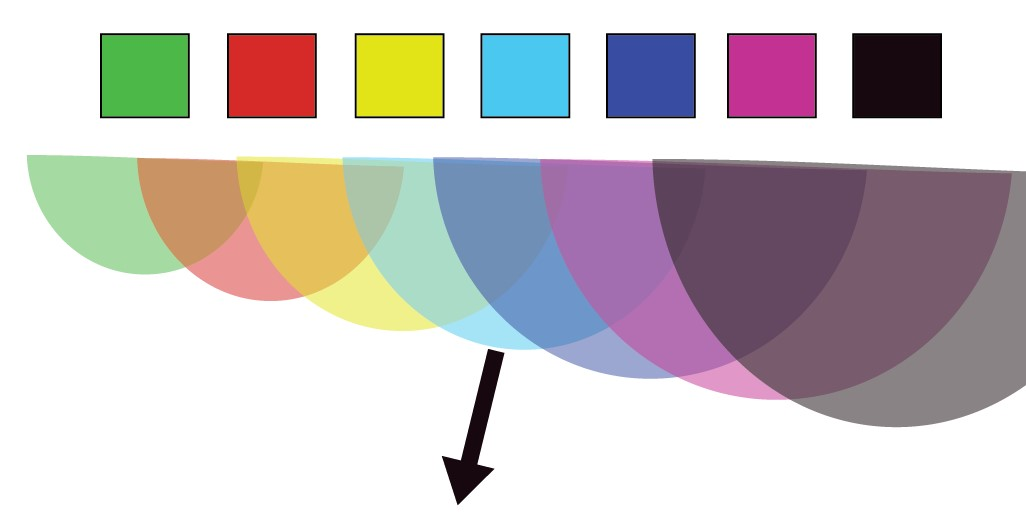
\includegraphics[width=\linewidth]{images/paa_bend}
				\caption{Delay estimation}
				\label{fig:bandwidth2}
			\end{minipage}
		\end{figure}
\end{frame}

\subsection{OBFN Chip}

\begin{frame}\frametitle{OBFN Chip}
		\begin{figure}
			\centering
			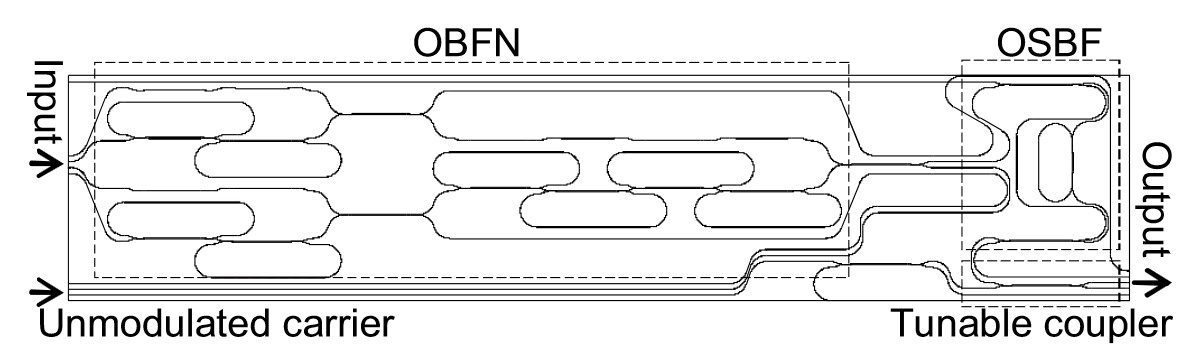
\includegraphics[width=0.8\linewidth]{images/OBFN_chip}
			\caption{Step response of open loop}
			\label{fig:bandwidth1}
		\end{figure}
\end{frame}

\subsection{Optical Ring Resonator (ORR)}

\begin{frame}\frametitle{Optical Ring Resonator (ORR)}
	\begin{figure}[H]
			\begin{minipage}[t]{0.4\textwidth}
				\centering
				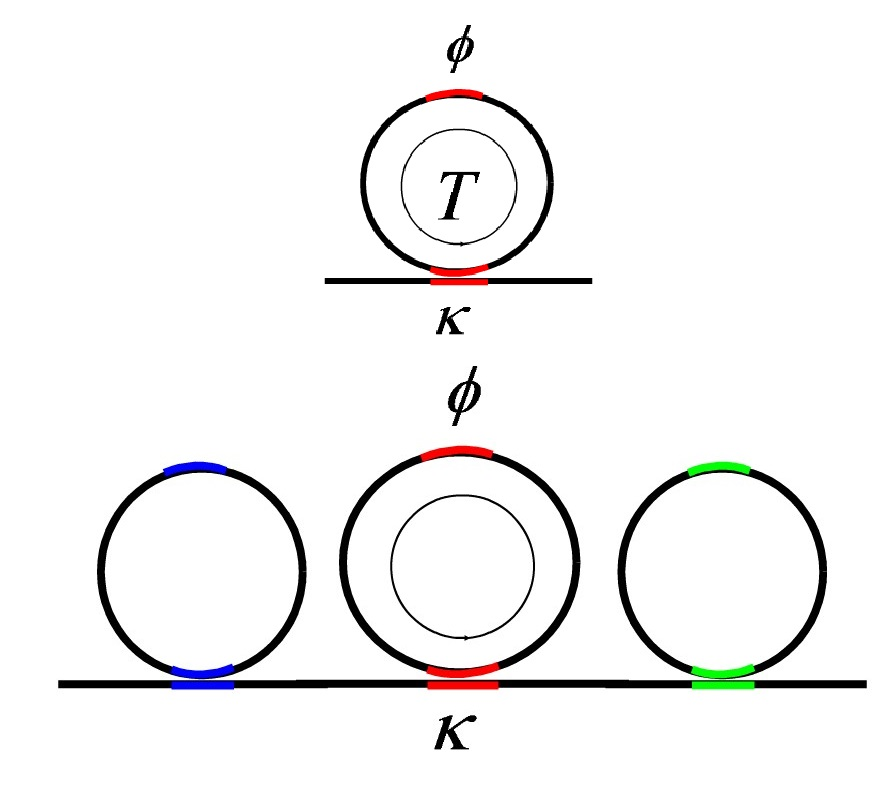
\includegraphics[width=\linewidth]{images/ORR}
				\caption{Step response of open loop}
				\label{fig:bandwidth1}
			\end{minipage}
				\hspace{\fill}
			\begin{minipage}[t]{0.55\textwidth}
				\centering
				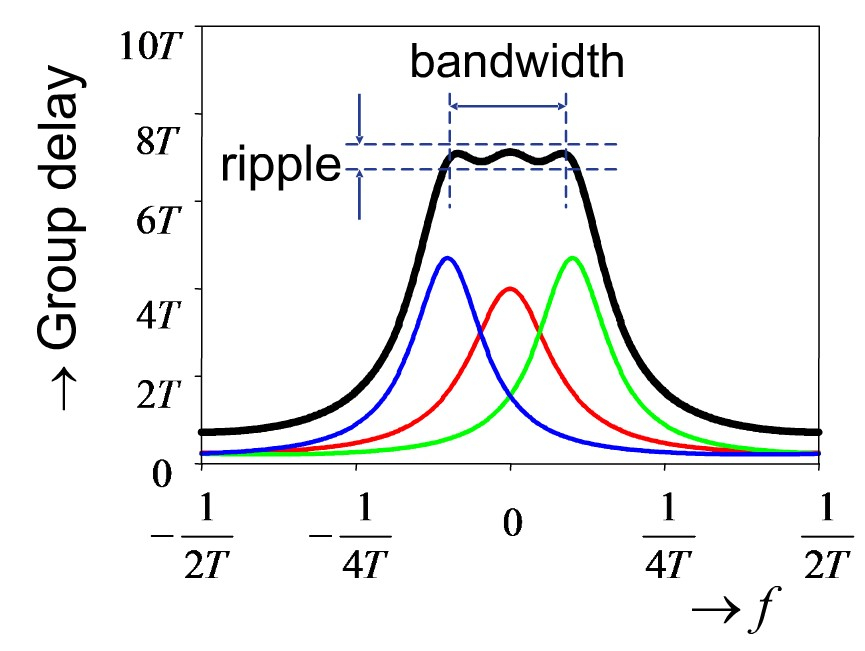
\includegraphics[width=\linewidth]{images/ORR2}
				\caption{Delay estimation}
				\label{fig:bandwidth2}
			\end{minipage}
	\end{figure}
\end{frame}

\section{Tuning of OBFN}

\subsection{Parameter to be Tuned}

\begin{frame}\frametitle{Parameters to be Tuned}

	\begin{figure}
			\centering
			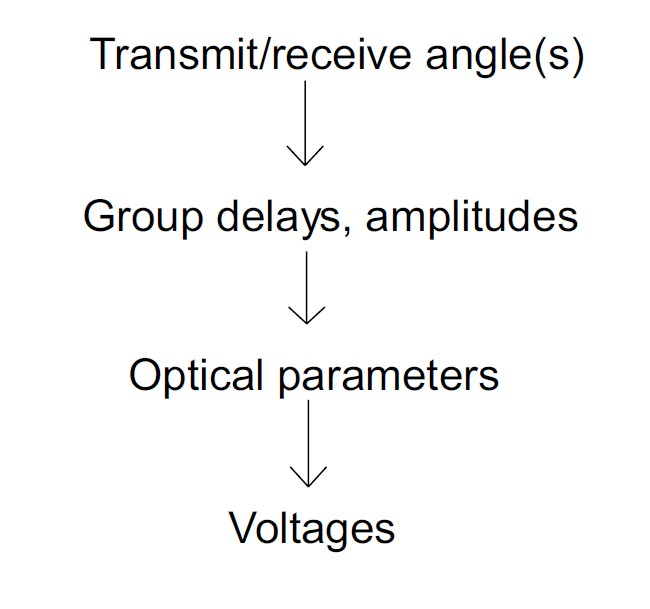
\includegraphics[width=0.35\linewidth]{images/project_layer}
			\caption{The Project layers}
			\label{fig:projlayers}
	\end{figure}
	\begin{alertblock}{Parameters to be Tuned: Optical Parameters}
		Parameters to be tuned to get the desired goals are the optical parameters : $\kappa$, $\theta$, and $T$ of each ORR\\
	\end{alertblock}
\end{frame}

\subsection{Desired Goals of Tuning}

\begin{frame}\frametitle{Desired Goals of Tuning}
	\begin{figure}
			\centering
			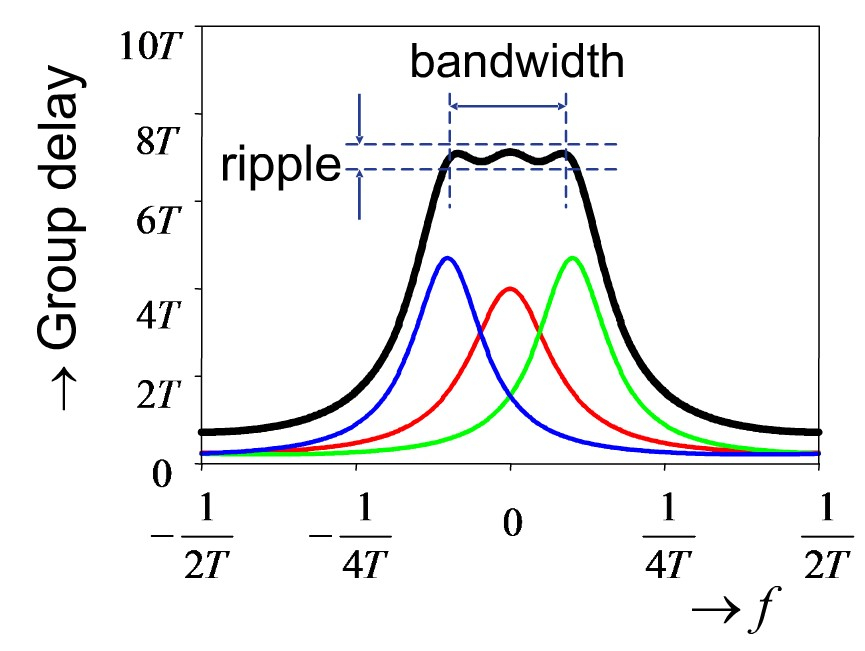
\includegraphics[width=0.45\linewidth]{images/ORR2}
			%\caption{The Project layers}
			\label{fig:projlayers}
	\end{figure}
	\begin{alertblock}{Goals: Group delays, ripple and bandwidth}
		Group delays : a certain value\\
		ripple : flat\\
		bandwidth : alligned with the spectrum of the modulated optical signal
	\end{alertblock}
\end{frame}

\subsection[]{Section 2 - Last Subsection}

\begin{frame}\frametitle{Last Page}
	\begin{block}{Summary}
		\centering{End of the beamer demo\\
		with a \emph{tidy} TU~Delft lay-out.\\
		Thank you!}
	\end{block}
\end{frame}

\end{document}
